\subsection{Etapa de abstracción}

Los recursos de FHIR se modelan dentro de un sistema de tipos de FHIR. Este último es similar a la formalización propuesta en \cite{Maldonado09}, la cual permite expresar los recursos de manera independiente a la sintaxis de FHIR conservando la estructura. En el formalismo de este trabajo se incluye la semántica de los recursos y se crean identificadores que más adelante se convertirán en los identificadores de los nodos de los arquetipos.

Una ventaja de que estos identificadores se mantengan en los arquetipos creados es la posibilidad de formar caminos ADL en esta etapa y relacionarlos con los nombres de los elementos de los recursos. Estas relaciones se podrán usar para convertir los datos desde su formato sintáctico original FHIR en estructuras openEHR por medio de programas de transformación basados en XQuery.

Las salidas de la abstracción, llamados esquemas FHIR, son conjuntos de tipos de FHIR definidos formalmente, los cuales modelan los recursos.

Como ejemplo, considerando el recurso SimplifiedPatient (Ver figura \ref{fig:abstraction} (a)) que es una simplificación del recurso Patient de FHIR, se puede abstraer dentro de un sistema de tipos de datos de FHIR (Ver figura \ref{fig:abstraction} (b)).

\begin{figure}
  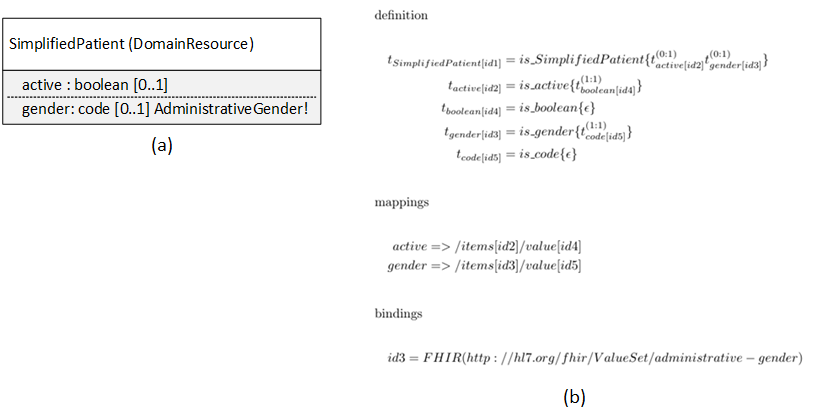
\includegraphics[scale=0.5]{./images/abstraction}
  \caption{(a) Recurso SimplifiedPatient (b) Esquema FHIR del recurso SimplifiedPatient}
  \label{fig:abstraction}
\end{figure}
